\documentclass[11pt,a4paper]{report}
\usepackage{afterpage}
\usepackage{hyperref}
\hypersetup{
colorlinks,
allcolors=black,
linktoc=all
}
\usepackage{titlesec}
%\titleformat{\chapter}[display]{\vspace{-3cm}\normalfont\bfseries}{}{0pt}{\LARGE}
%\titleformat{\chapter}[display]
%  {\normalfont\huge\bfseries}{\chaptertitlename\ \thechapter}{5pt}{\Huge}
%\titleformat{\section}
%  {\normalfont\Large\bfseries}{\thesection}{1em}{}
%\titleformat{\subsection}
%  {\normalfont\large\bfseries}{\thesubsection}{1em}{}
%\titleformat{\subsubsection}
%  {\normalfont\normalsize\bfseries}{\thesubsubsection}{1em}{}
%\titleformat{\paragraph}[runin]
%\  {\normalfont\normalsize\bfseries}{\theparagraph}{1em}{}
%\\titleformat{\subparagraph}[runin]
%\  {\normalfont\normalsize\bfseries}{\thesubparagraph}{1em}{}
  
\usepackage[english,main=spanish]{babel}
\usepackage[utf8]{inputenc}
\usepackage{color}
\usepackage[table]{xcolor}
\usepackage{graphicx}
\usepackage[export]{adjustbox}
\usepackage{amssymb}
\usepackage{url}
\usepackage{xcolor}
\usepackage{caption}
\usepackage{float}
\usepackage{listingsutf8}
\usepackage[framemethod=default]{mdframed}
\definecolor{LightGray}{gray}{0.9}
\usepackage{babel}
\usepackage[english]{babelbib}


\definecolor{codegreen}{rgb}{0,0.6,0}
\definecolor{codegray}{rgb}{0.5,0.5,0.5}
\definecolor{codepurple}{rgb}{0.58,0,0.82}
\definecolor{backcolour}{rgb}{0.95,0.95,0.92}
\usepackage{caption}
\usepackage{subcaption}
\lstdefinestyle{codigo}{
    backgroundcolor= \color{backcolour},   
    commentstyle=\color{codegreen},
    keywordstyle=\color{magenta},
    numberstyle=\tiny\color{codegray},
    stringstyle=\color{codepurple},
    basicstyle=\scriptsize\normalfont\sffamily,  
    breakatwhitespace=false,         
    breaklines=true,                 
    captionpos=t,                 
    keepspaces=true,
    numbers=left,                   
    numbersep=5pt,  
    showspaces=false,                
    showstringspaces=false,
    showtabs=false,                  
    tabsize=2,
    frame=single,
    framexleftmargin=15pt,
    framexrightmargin=5pt,
    framexbottommargin=5pt,
    framextopmargin=5pt,
    inputencoding=utf8,
    extendedchars=true,
    literate = {¬}{{$\neg$}}1
}

\DeclareCaptionFormat{listing}{#1#2#3}
\captionsetup[lstlisting]{format=listing,singlelinecheck=false, margin=0pt, font={sf},labelsep=space,labelfont=bf}


\renewcommand{\lstlistingname}{Código}
\renewcommand{\lstlistlistingname}{Índice de códigos}

\usepackage[many]{tcolorbox}  
\newtcolorbox{boxB}{
    boxrule = 1.5pt,
    colframe = white,
    rounded corners,
    arc = 5pt
}

\definecolor{mygreen}{rgb}{0,0.6,0}
\definecolor{mygray}{rgb}{0.5,0.5,0.5}
\definecolor{mymauve}{rgb}{0.58,0,0.82}
\definecolor{terminalbgcolor}{HTML}{330033}
\definecolor{terminalrulecolor}{HTML}{000099}

\lstdefinestyle{terminal}
{
    backgroundcolor=\color{black},
	basicstyle=\scriptsize\color{white}\ttfamily,
	breaklines=true,
	captionpos=t,
	extendedchars=true,
	showspaces=false,
	showstringspaces=false,
	frame=single,
    framexleftmargin=5pt,
    framexrightmargin=5pt,
    framexbottommargin=5pt,
    framextopmargin=5pt,
    breakindent=0pt,
    breakautoindent=false,
    literate={\$}{{\$}}1 
         {:}{{:}}1
         {¬}{{$\neg$}}1
         {~}{{\textasciitilde}}1,
}

\begin{document}

\begin{titlepage}
\begin{center}
\LARGE
\textbf{Comparación de algoritmos MPPTs en sistema real}

\vspace{0.4cm}
Trabajo Final en Electrónica

\vspace{0.5cm}
\textbf{Pablo Agustín Nievas Aramayo}

\vspace{0.3cm}
\small
\textbf{Director de Trabajo Final}: Castagnola, Juan\\
\textbf{Subdirector de Trabajo Final}: Petrashin, Pablo

\vspace{0.4cm}


\includegraphics[scale=0.5]{imagenes/FacuIcon.png}

\Large
Facultad de Ingeniería Electrónica\\
\end{center}
\end{titlepage}
\pagenumbering{roman} 
\chapter*{Declaratoria de Autoría}
\thispagestyle{empty}
Yo, Pablo Agustín Nievas Aramayo, declaro que el trabajo que se presenta en esa obra es de mano propia. Puedo asegurar que:

\begin{itemize}
 
\item La obra fue producida en su totalidad mientras realizaba el Trabajo Final

\item Cuando se ha consultado el trabajo publicado por otros, lo he atribuido con claridad;
\item Cuando se ha citado obras de otros, he indicado las fuentes. Con excepción de estas citas, la obra es enteramente mía;
\item Cuando la obra se basa en trabajo realizado conjuntamente con otros, he explicado claramente qué fue contribuido por otros, y qué fue contribuido por mi;
\item Ninguna parte de este trabajo ha sido publicada previamente a su entrega, excepto donde se han realizado las aclaraciones correspondientes. Capaz que esto es incorrecto debido al Paper

\end{itemize}

\vspace{0.5cm}

\begin{figure}[h]
\centering
\begin{subfigure}{0.5\textwidth}
  \centering
  
\includegraphics[width=1\linewidth]{imagenes/Firma.png}\\
   Pablo Agustín Nievas Aramayo\\
   17/8/2022 Actuaizar esta fecha
  \label{fig:sub1}
\end{subfigure}%
\label{fig:test}
\end{figure}   %camiar a imagen del profe de firmar?
%\afterpage{\null\thispagestyle{empty}\newpage}
\chapter*{Motivacón}
\markboth{Motivacón}{Motivacón}
\thispagestyle{empty}
Una de las motivaciones mas grandes a la hora de realizar este trabajo final es George Russel Harrion. Después de leer su libro "Átomos en acción", y ver como muchas de sus palabras son relevantes en la actualidad despertó mi visión de que algo tenia que hacer con mis conocimientos y la energía renovable.  Incluso para un libro escrito en el año 1942, su visión de energía y física creadora es realista y posible. Solo hay que tomar acción.Espero que este trabajo final sea el primer paso para mi maratón de energía libre.    
\chapter*{Agradecimientos}
\markboth{AGRADECIMIENTOS}{AGRADECIMIENTOS}
\thispagestyle{empty}
Este trabajo no habría sido posible sin el apoyo del profesor Pablo Petrashin,  bajo cuya supervisión escogí este tema y comencé la tesis. Director Juan Castagnola, mi consejero en las etapas finales
del trabajo, también ha sido generosamente servicial, y me ha ayudado de
numerosos modos.
No puedo terminar sin agradecer a mi familia, en cuyo estímulo constante y
amor he confiado a lo largo de mis años en la Academia. Estoy agradecido
también a los ejemplos de mis  familiares, que recorren el mismo camino del conocimiento. Es a ellos, tanto como a los difuntos y por nacer, que dedico este trabajo.     
\setcounter{page}{1}
\tableofcontents


\listoftables
%\lstlistoflistings


\listoffigures


\setcounter{page}{1}
\chapter*{Resumen}
\addcontentsline{toc}{chapter}{Resumen}
\pagenumbering{arabic} % And moving back to arabic numbering (1,2,3,4) for the body.
\patchcmd{\chapter}
  {\clearpage}
  {\cleardoublepage}
  {}
  {}
Con la emergente onda que parece no detenerse, la energía solar no deja de crecer, tanto como los avances tecnológicos alrededor de ésta, como el número de lugares donde se encuentran estas fuentes de energía. 

Sin embargo, para conectar de manera correcta los paneles solares es necesario un control electrónico entre éstos y la respectiva carga para obtener el punto de máxima potencia y eficiencia. 

Se destacan dos partes en el control de potencia de paneles solares:

La primera, la topología de los posibles circuitos de electrónica de potencia que uno puede emplear. De estas topologías hay desde hace 50 años, sin embargo, el desarrollo de nuevas topologías nunca se detuvo.

La segunda, la metodología de los algoritmos que buscan el punto de máxima potencia (\textit{Máximum Power Point Tracking}, MPPT). Al igual que las topologías de circuitos de control para paneles solares, estos métodos existen desde hace años, y hay metodologías emergentes en el estado del arte.

Al realizar la combinación de estas dos partes en un sistema de paneles fotovoltaicos se obtiene el completo control electrónico de la energía que brinda esta fuente.

Por lo que en el presente trabajo, se realiza el desarrollo, diseño, análisis e implementación de la topología del conversor síncrono DC-DC reductor (\textit{Buck}, \textit{Stepdown}) junto con metodologías de perturbación y observación (\textit{Perturb and Observe}, P\&O) modificadas.

La implementación de las metodologías es sobre la placa de desarrollo ESP32 (\textit{DeveloperBoard}) y la recolección de datos se almacenan en una hoja de cálculo en internet utilizando las herramientas de Google.    




\chapter{Introducción}
\label{Introducción}

%Historia de como se presenta la oportunidad de hacer este trabajo final
Ante la propuesta del profesor Petrashin de desarrollar un trabajo final en base al tema presentado en microelectrónica II, Control Potencia con circuitos integrados (\textit{Power Management Integrated Circuits, PMIC}), se desarrolla el presente trabajo final. Partiendo de tesis de doctorado (referencia) se realiza una investigación del estado del arte y se estudia los conversores DC-DC. Por lo que se delimita el alcance del Trabajo Final con los requerimientos funcionales y no funcionales.
\section{Requerimientos Funcionales y No funcionales}
Para poder realizar el trabajo dentro de un tiempo comprensible, y no tenga un alcance ¿uperior/desviado al titulo de ingeniero electrónico, se pauta la tabla \ref{requerimientos-tabla}.
\begin{table}[h]
\resizebox{\textwidth}{!}{\begin{tabular}{|c|c|c|}
    \hline
    Requerimientos Funcionales & Requerimientos No Funcionales\\
    \hline
    Potencia máxima de panel solar de 300W & Emplear un conjunto de paneles solares de la universidad UCC\\
    \hline
    Corroborar distintos métodos de MPPT & Disponibilidad local de componentes\\
    \hline
    Guardar los datos reales & Fácil instalación y replica\\
    \hline
\end{tabular}}
\caption{Requerimientos funcionales y no funcionales}
\label{requerimientos-tabla}
\end{table}

\section{Zona de trabajo}
Se desarrolla el trabajo teniendo en cuenta que se implementa/implementara en el sector de energías renovables en el exterior de la facultad de ingenierías de la Universidad Católica de Córdoba. Un sector aislado del edificio ubicado en las coordenadas -31.486791, -64.240144. Los paneles presentes son de código KS75T de la empresa SOLARTEC®, Figura \ref{fig:panelsolarencampo}, cuya curva característica de potencia se observa en la Figura \ref{fig:curvadepaneldata}
\begin{figure}
    \centering
    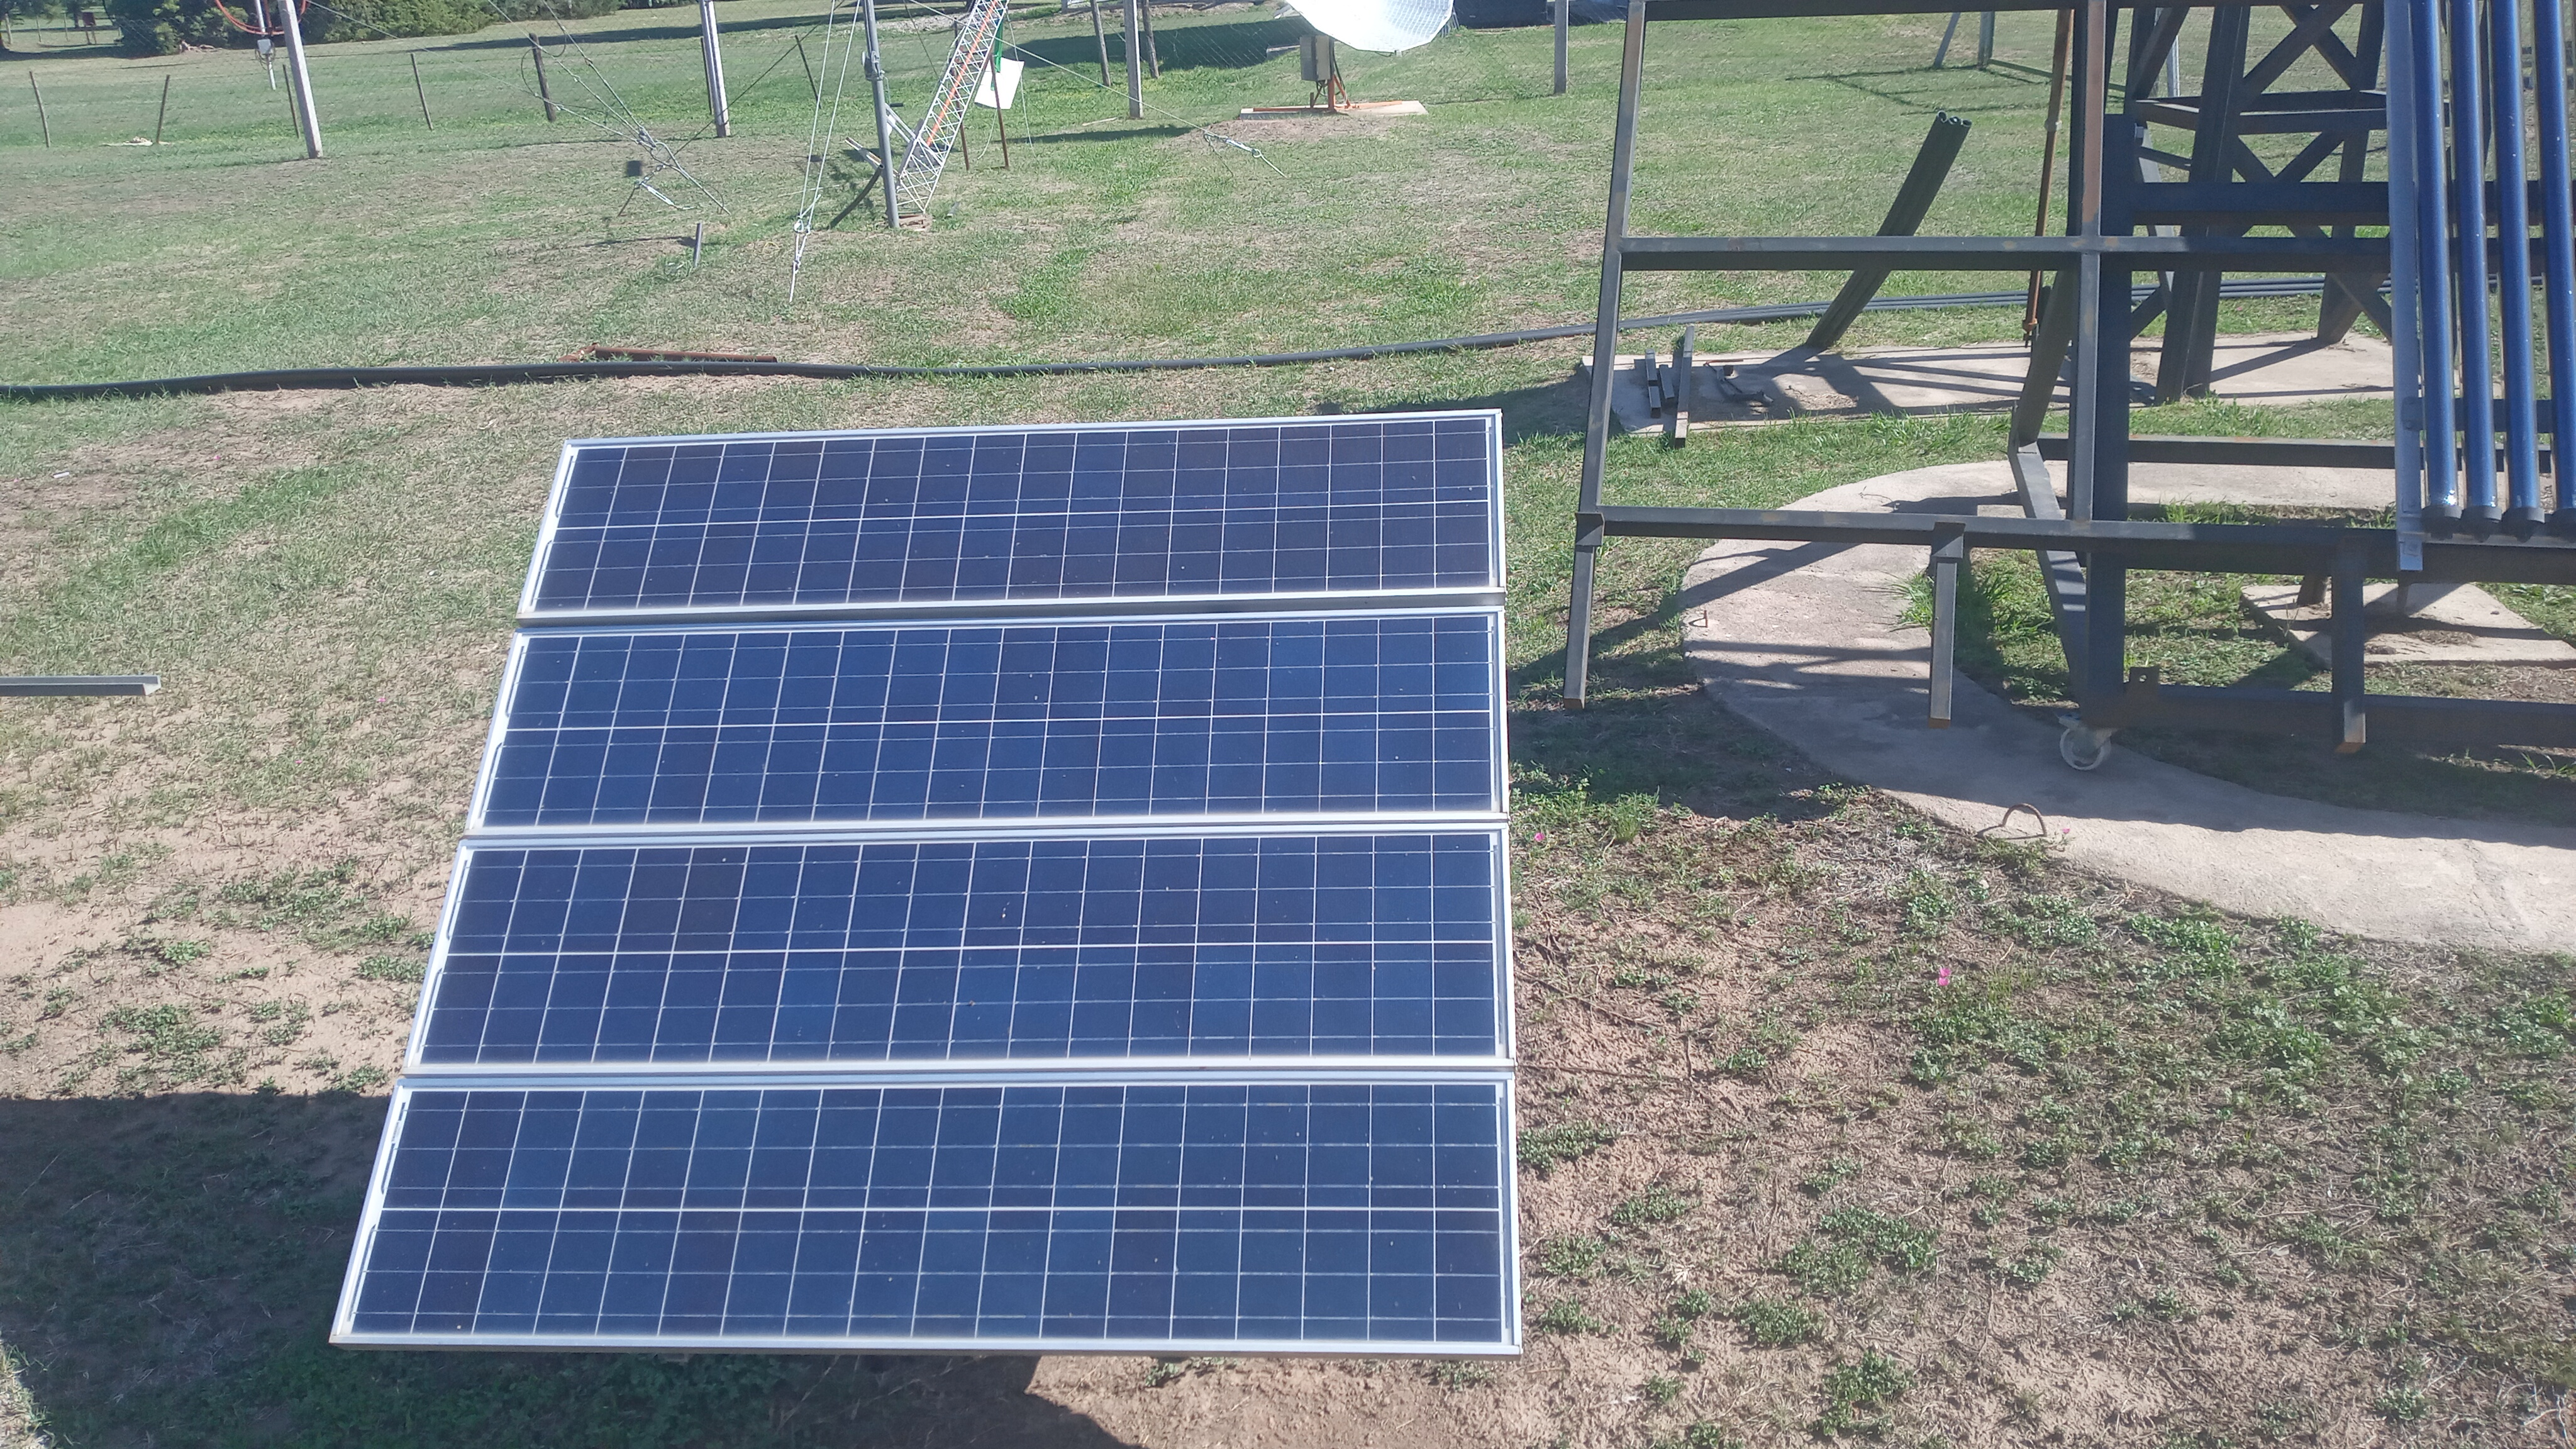
\includegraphics[width=1\linewidth,frame]{imagenes/panelsolarencampofrontal.jpg}
    \caption{Paneles solares en campo}
    \label{fig:panelsolarencampo}
\end{figure}
\begin{figure}
    \centering
    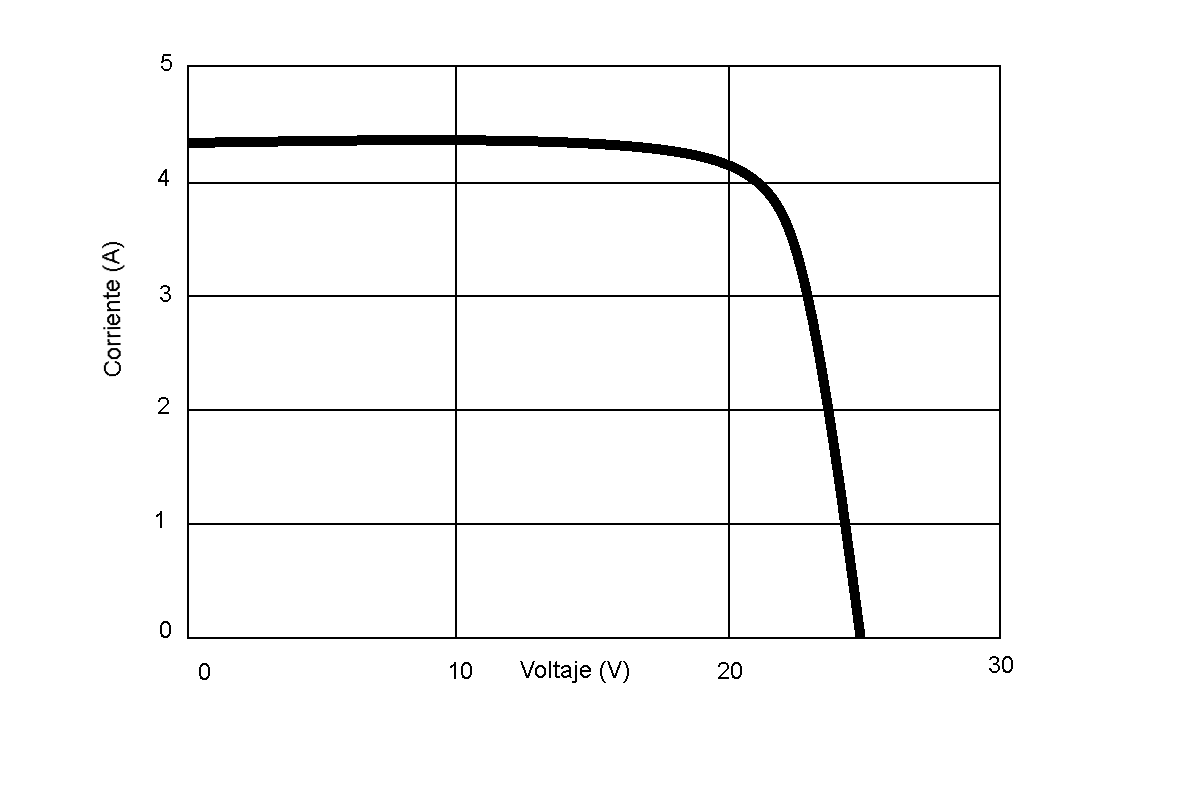
\includegraphics[width=1\linewidth,frame]{imagenes/curvapaneldata.png}
    \caption{Curva característica de Panel Solar}
    \label{fig:curvadepaneldata}
\end{figure}

\chapter{Fundamentación Teórica. Electrónica y Computación}
\label{teoria}
La teoría que se puede aplicar a los componentes del sistema a implementar en este trabajo pueden ser bastante complejos. Sin embargo, no es necesario un análisis profundo en un sistema de control de panel solar con una carga resistiva. Por lo que se explica solo lo necesario para el comprender del funcionamiento y razón sobre la elección de los componentes en un sistema real.
\section{Electrónica de Potencia}
Para realizar un control de potencia en continua, la electrónica emplea componentes semiconductores (Figura \ref{fig:semicon}) en circuitos llamados Conversores DC-DC (Figura \ref{fig:topologiassimples}).
\begin{figure}[H]
    \centering
    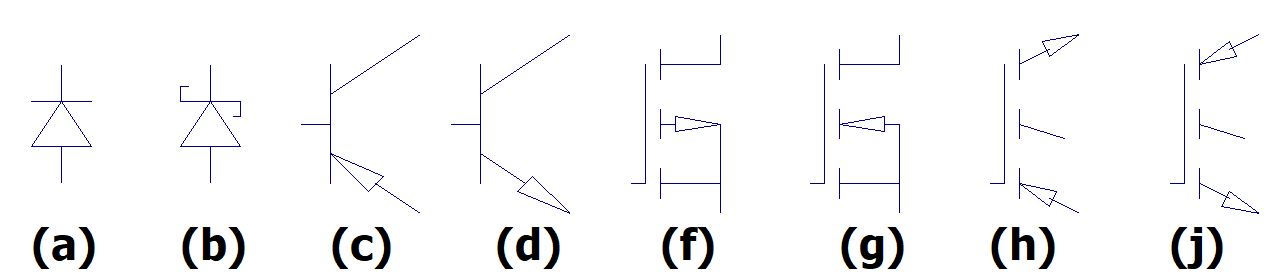
\includegraphics[width=\linewidth]{imagenes/semiconductores.png}
    \caption{Interruptores unipolares de acción simple: (a) Diodo simple, (b) Diodo Schottkey, (c) Transistor BJT tipo P y (d) tipo N, (f) Mosfet tipo P y (g) N, (h) IGBT tipo P y (j) N}
    \label{fig:semicon}
\end{figure}

\begin{figure}[H]
    \centering
    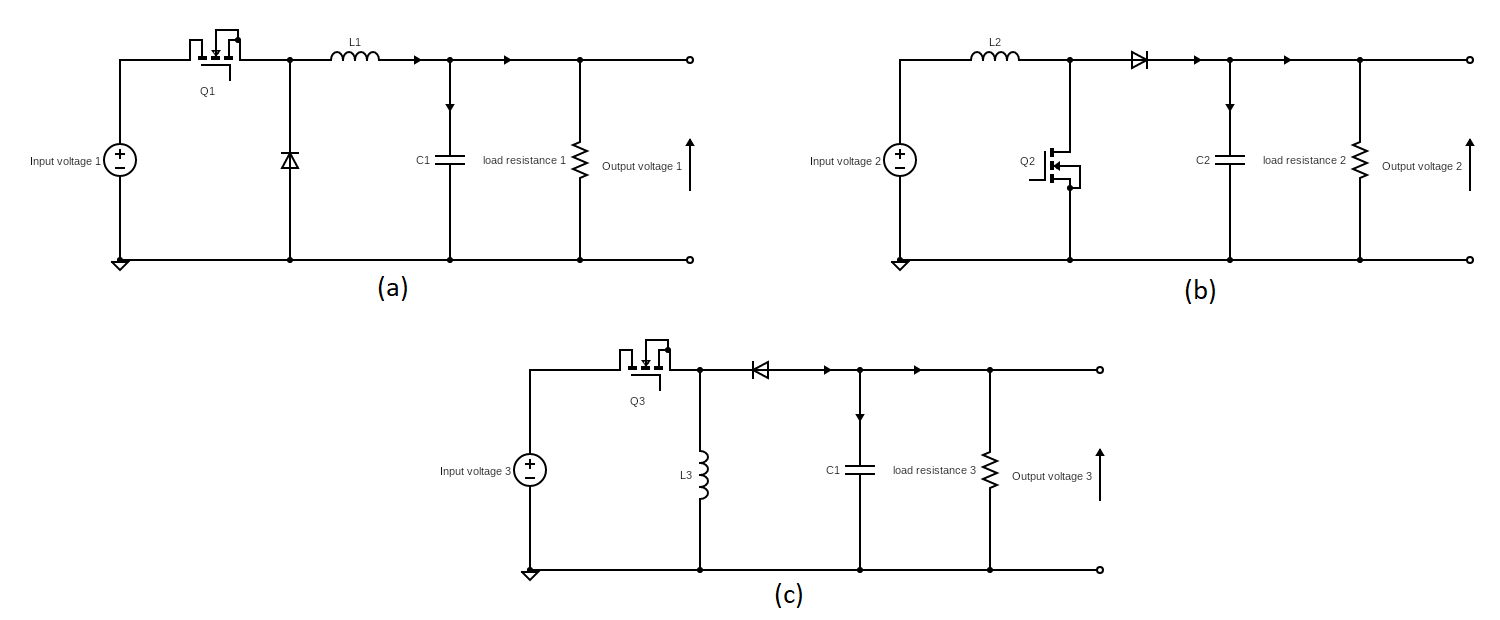
\includegraphics[width=\linewidth]{imagenes/simpletopologies.png}
    \caption{Conversores DC-DC no aislados: (a) Buck, (b) Boost, (c) Buck-Boost}
    \label{fig:topologiassimples}
\end{figure}
Obviamente, no son los únicos circuitos conversores DC-DC existentes los ilustrados en la figura \ref{fig:topologiassimples}, sino los mas simples de implementar matemática y físicamente hablando. El desarrollo de este tipo de conversores continua actualmente \cite{power}, pero la implementación de estos se escapa del alcance del presente trabajo.\par La elección de que topología utilizar de la Figura \ref{fig:topologiassimples} dependerá de la respuesta deseada del sistema.
\subsection{Semiconductores}
Los dispositivos semiconductores en potencia se comportan como interruptores unipolares de acción simple, y dependiendo de los parámetros deseables en la implementación es la elección de uno sobre otro. 
\subsubsection{Diodo}
El diodo es un semiconductor de materiales n y p 
El diodo entra en estado de polarización al conectarle en los contactos una tensión. Dependiendo de la tensión es una polarización directa o inversa.\par \par Unas de las mayores ventajas de los diodos Schottky es su rápida velocidad de conmutación y una baja caída de voltaje al estar polarizado en modo directo. Incluso el tiempo transitorio de recuperación inversa no es importante. Sin embargo, pocos dispositivos comerciales superan una tensión de ruptura de 100V. Por lo que son preferibles ante sistemas de bajo voltaje (45V o menos). Otro problema es que la corriente de fuga mayor que la de un diodo de silicio comparable \cite{power}.\par 
\subsubsection{MOSFET}
Mosfet rapido veloz
\subsection{Conversores DC-DC}

    
\subsubsection{Buck Síncrono}
\begin{equation} \label{potin}
	P_{in} = {V_{in} \times  I_{in}}
	\end{equation}
\begin{equation} \label{potout}
	 P_{out} = {V_{out} \times  I_{out}} 
\end{equation}
\begin{equation} \label{potineqpotout}
	 P_{in}\times\eta = P_{out}
\end{equation}
\begin{equation} \label{potinaproxpotout}
	 P_{in}\approx P_{out}
\end{equation}
\begin{equation} \label{voutvioniiniout}
	 {V_{in} \times  I_{in}} = {V_{out} \times  I_{out}} 
\end{equation}
\begin{equation} \label{vinDvout}
	 {V_{in} \times  D} = {V_{out} } 
\end{equation}
\begin{equation} \label{iinioutd}
	{ I_{in} \times \frac{1}{D}} = {I_{out}} 
\end{equation}
\begin{equation} \label{limitesded}
	{0\leq D \leq 1}
\end{equation}
\begin{equation} \label{rinprima}
	{ R_{in}'} = {\frac{V_{in}}{I_{in}}} 
\end{equation}
\begin{equation} \label{routprima}
	{ R_{out}} = {\frac{V_{out}}{I_{out}}} 
\end{equation}
\begin{equation} \label{rinandrouteq}
	{ R_{in}'\times I_{in} \times I_{in}} = {R_{out}\times I_{out} \times I_{out}} 
\end{equation}
\begin{equation} \label{rinroutsquare}
	{ R_{in}'\times I_{in}^2} = {R_{out}\times I_{out}^2} 
\end{equation}
\begin{equation} \label{rinroutsquareoniinonesquare}
	{ R_{in}'\times I_{in}^2} = {R_{out}\times (\frac{I_{in}}{D})^2} 
\end{equation}
\begin{equation} \label{rinroutsquareoniin}
	{ R_{in}'\times I_{in}^2} = {R_{out}\times I_{in}^2 \times \frac{1}{D^2}} 
\end{equation}
\begin{equation} \label{rinroutalmostfinal}
	{ R_{in}'} = {R_{out}\times \frac{1}{D^2}} 
\end{equation}
\begin{equation} \label{rinroutfinal}
	{D} = {\sqrt{\frac{R_{out}}{R_{in}'}}} 
\end{equation}
\begin{equation} \label{routlessrin}
	R_{out}<R_{in}'
\end{equation}
\begin{equation} \label{rinbaseonrout}
	R_{in}'={\frac{R_{out}}{D^2}}
\end{equation}
\begin{equation} \label{frecuenciadetanke}
	f_c={\frac{1}{2\times \pi \times \sqrt{L\times C}}}
\end{equation}
\begin{equation} \label{fcmenorfs}
	f_c<<f_s
\end{equation}
\begin{equation} \label{fcmayorfs}
	f_c>>f_s
\end{equation}
\begin{equation} \label{deltail}
	\Delta I_L={\frac{V_{in}\times D \times(1-D)}{f_s\times L}}
\end{equation}
\begin{equation} \label{deltavc}
	\Delta V_c={\frac{V_{in}\times D \times(1-D)}{8\times f_s^2\times L \times C}}
\end{equation}
\begin{equation} \label{calculodeinductancia}
	L={\frac{V_{out} \times(1-D)}{f_s\times \Delta I_L}}
\end{equation}
\begin{equation} \label{calculodecapacitancia}
	C={\frac{\Delta I_L}{8\times f_s\times \Delta V_c}}
\end{equation}
\begin{equation} \label{riplevout}
	{\frac{\Delta V_out}{V_out}}={\frac{\Delta I_L}{8\times f_s\times \Delta V_c}}
\end{equation}
\begin{figure}[H]
    \centering
    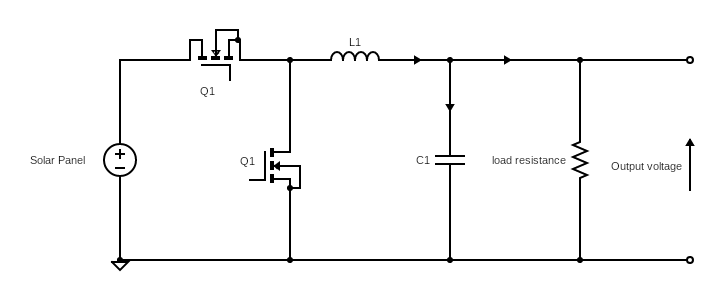
\includegraphics[width=1\linewidth,frame]{imagenes/syncbuck.png}
    \caption{Circuito de conversor Buck síncrono}
    \label{fig:circuito_final}
\end{figure}
\section{Paneles Solares}

\subsection{MPPT}

\subsection{Computación de MPPT}
El control en conversores DC-DC se da con una retroalimentación de tensión o corriente\cite{fundamental}, utilizando un circuito analógico generalmente para producir una tensión o corriente de salida estática. Sin embargo, para el control de sistemas fotovoltaicos, se emplea un control dinámico para obtener la máxima potencia, siendo este posible analógicamente en algunos casos, o dependientes de un sistema computacional. \par Los algoritmos de MPPT siguen evolucionando\cite{power}, sin embargo, se estudia el método básico de P\&O juntos con unas modificaciones.
\section{ESP32}
\subsection{MCPWM}

%\chapter{Apartado Metodológico}
\label{Apartado Metodológico}

Imagen de ejemplo.

\begin{figure}[H]
\begin{center}

\includegraphics[width=1\linewidth,frame]{imagenes/solar-icon.png}
\caption{Esta es una imagen}
\label{solaricon}
\end{center}
\end{figure}
\chapter{Diseño e Implementación}
\label{Diseño e Implementación}
Todo paso por paso de peor a mejor
\section{Conversor Buck}
\subsection{Inductancia y Capacitancia}
\subsection{Mosfet}
\section{Driver IR2110}
\section{Sensores}
\section{Método P\&O}
\section{Modificaciones en campo}
\subsection{Limitaciones de Inductor en Toroide}
\subsection{Protección de corriente en IR2110}
\subsection{Reducción de ruido}
\subsection{Modificación de método P\&O}
\section{Implementación del sistema}
\begin{figure}
    \centering
    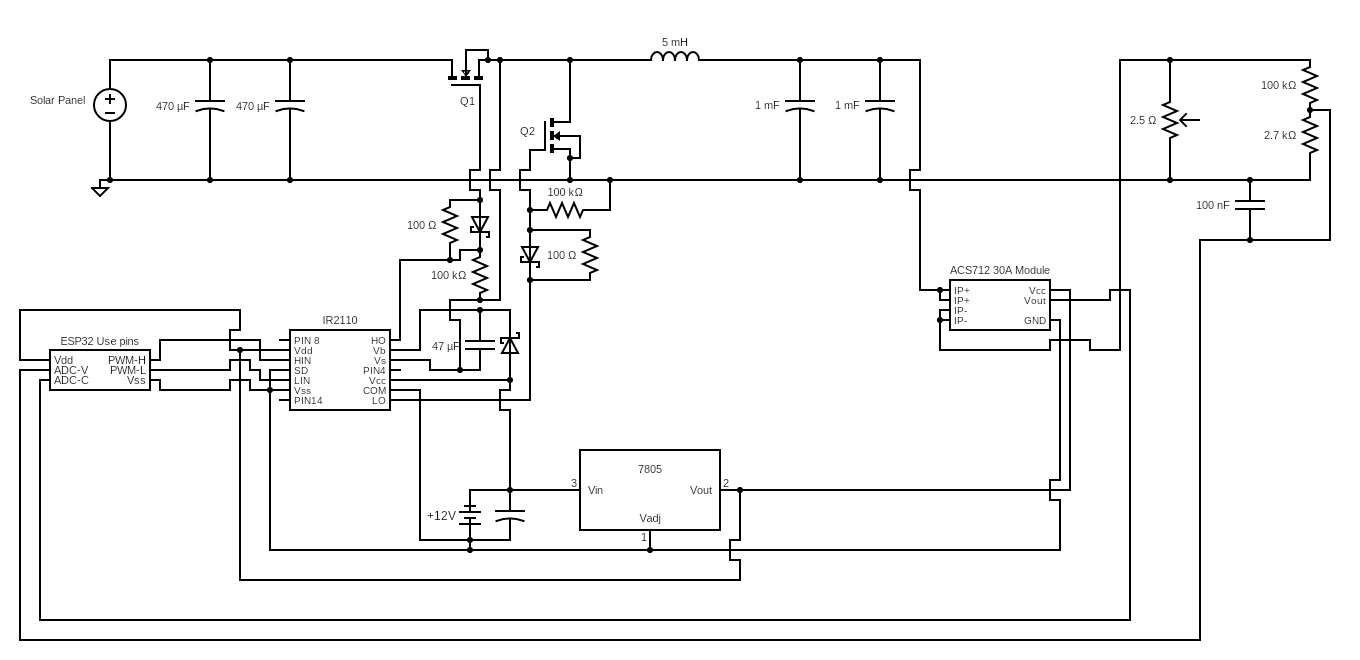
\includegraphics[width=1\linewidth,frame]{imagenes/finalcircuit.png}
    \caption{Esquemático de circuito final V1}
    \label{fig:circuito_final_circuit_diagram_org}
\end{figure}
\begin{figure}
    \centering
    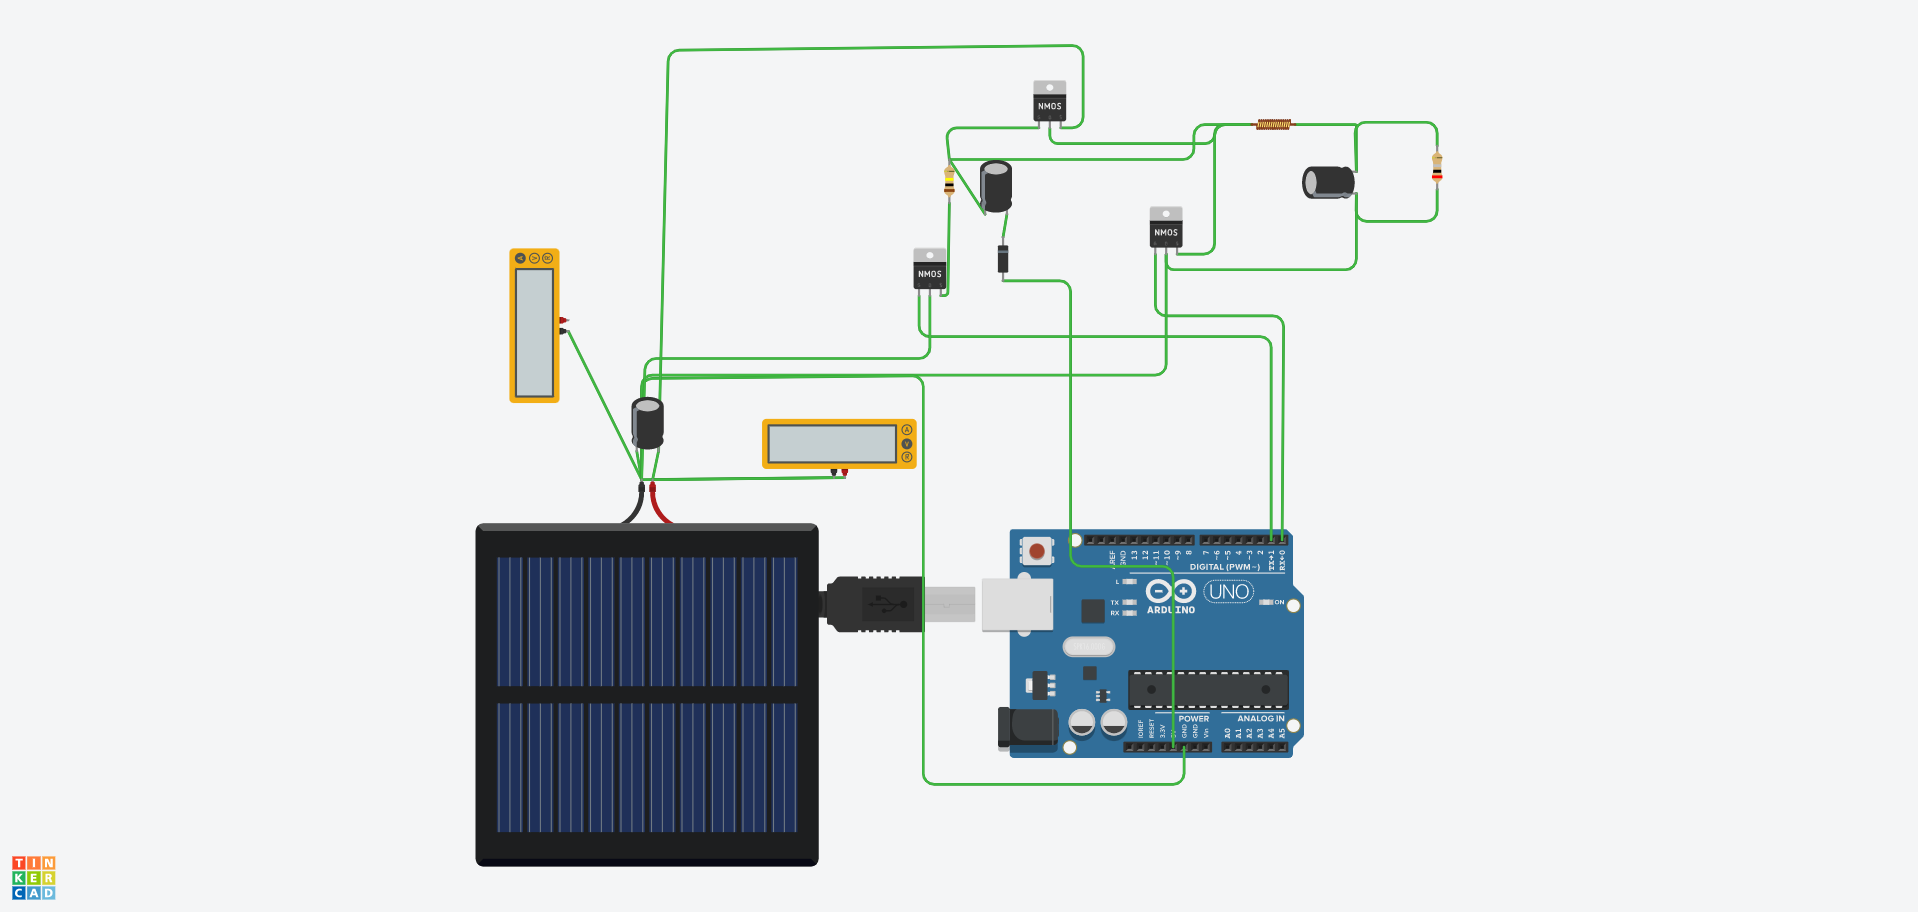
\includegraphics[width=1\linewidth,frame]{imagenes/testdecircuitoonline.png}
    \caption{Esquemático de circuito final V2}
    \label{fig:circuito_final_de_mentira}
\end{figure}
\chapter{Resultados Experimentales y Discusión}
\label{Resultados Experimentales y Discusión}
\section{Comportamiento de Conversor}
Esto es solo texto para ver el espacio de texto disponible para escribor. Aca se explicara como la resistencia de 100 Ohms ayuda a que el sobrepulso no romba el gate  del mosfet p
\begin{figure}[h!]
    \centering
    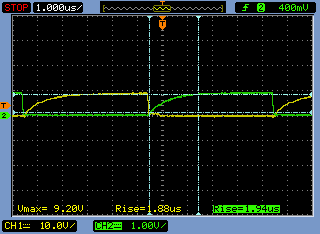
\includegraphics[width=1\linewidth]{imagenes/testosc0.png}
    \caption{Voltaje en Gate de Mosfets}
    \label{fig:tension_gate_mosfets}
\end{figure}
or estres, bajar el ruido, y baja la corriente exigida al driver. Tambien se explica como la resistencia de 10 Ohm quemo el driver. Como se ve en el impreso, imagenes ocupan bastante espacio si se deja al ratio de el ancho de escritura.
\subsection{Respuesta transitoria}
\begin{figure}[H]
    \centering
    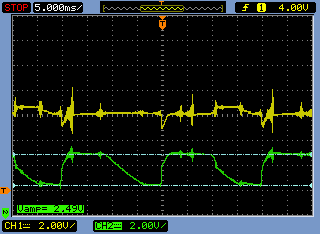
\includegraphics[width=1\linewidth,frame]{imagenes/testosc4.png}
    \caption{Respuesta transitoria de conversor en Laboratorio}
    \label{fig:resp_tran_lab}
\end{figure}
\section{Eficiencia}
La eficiencia del conversor Buck esta ligada al duty-cycle que le controla, por lo que un barrido de este conectado en el panel solar de campo se obtiene la figura \ref{fig:efficiency_solar_panel}.
\begin{figure}[H]
    \centering
    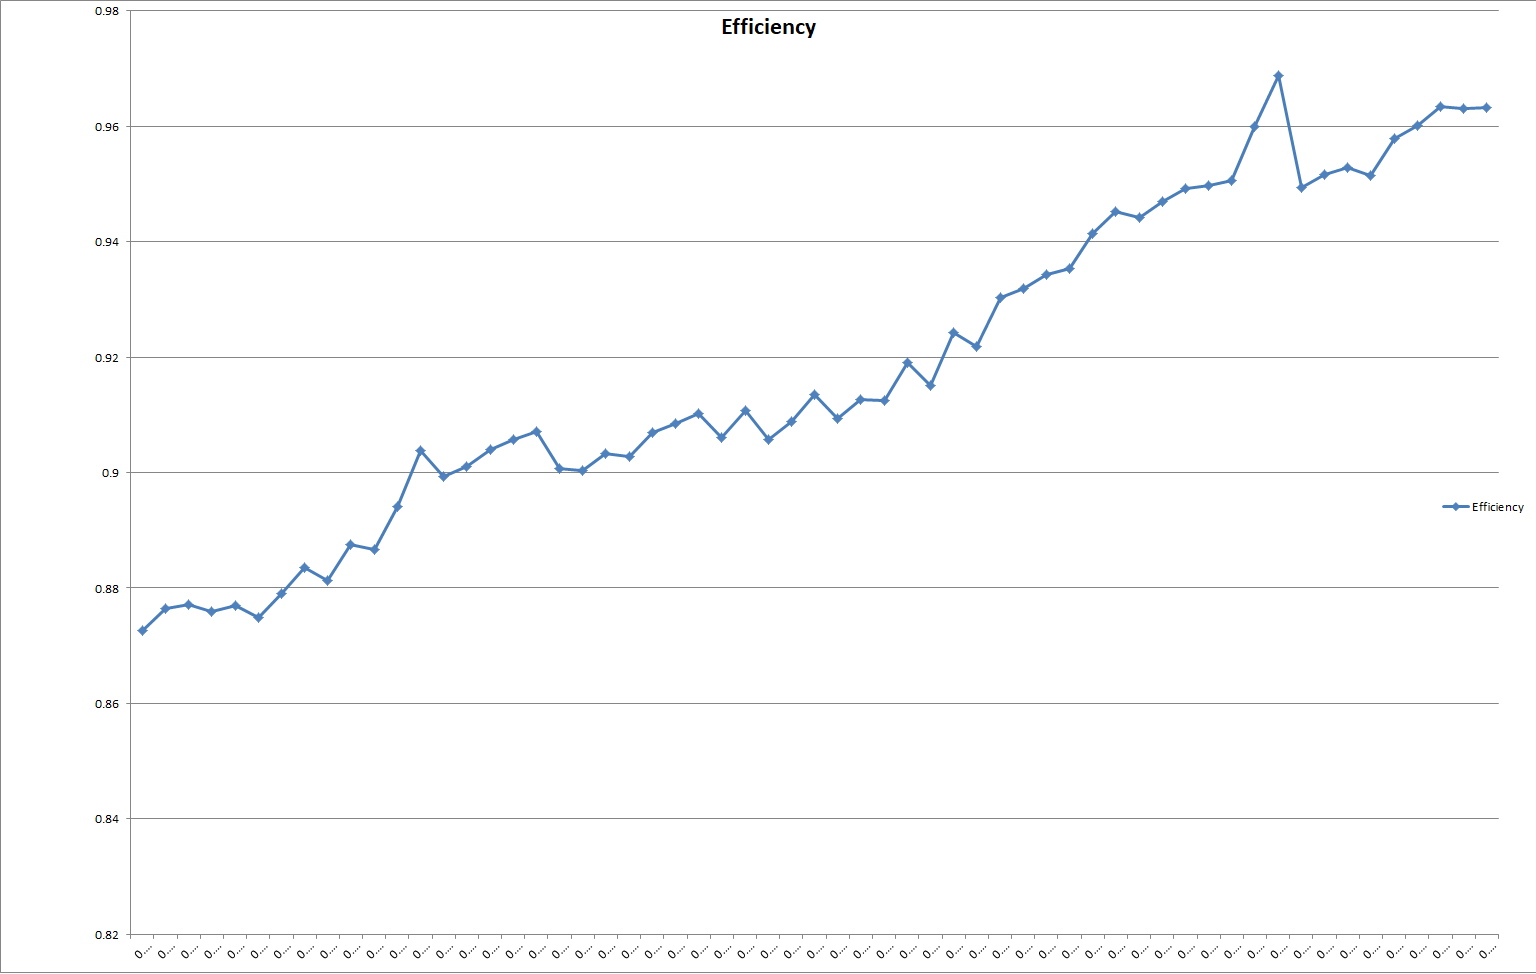
\includegraphics[width=1\linewidth]{imagenes/efficiency.png}
    \caption{Eficiencia de conversor Buck en campo}
    \label{fig:efficiency_solar_panel}
\end{figure}
\section{Condición de sombreado parcial}
\section{Respuesta de los métodos MPPT}
Con un barrido de duty-cycle en sistema real a través de la placa esp32 ,y calculo en tabla de excel posterior, se realiza las conclusiones, desarrollo, y modificaciones a los métodos en base a la curva de la Figura \ref{fig:curva_panel_esp32}.
\begin{figure}[H]
    \centering
    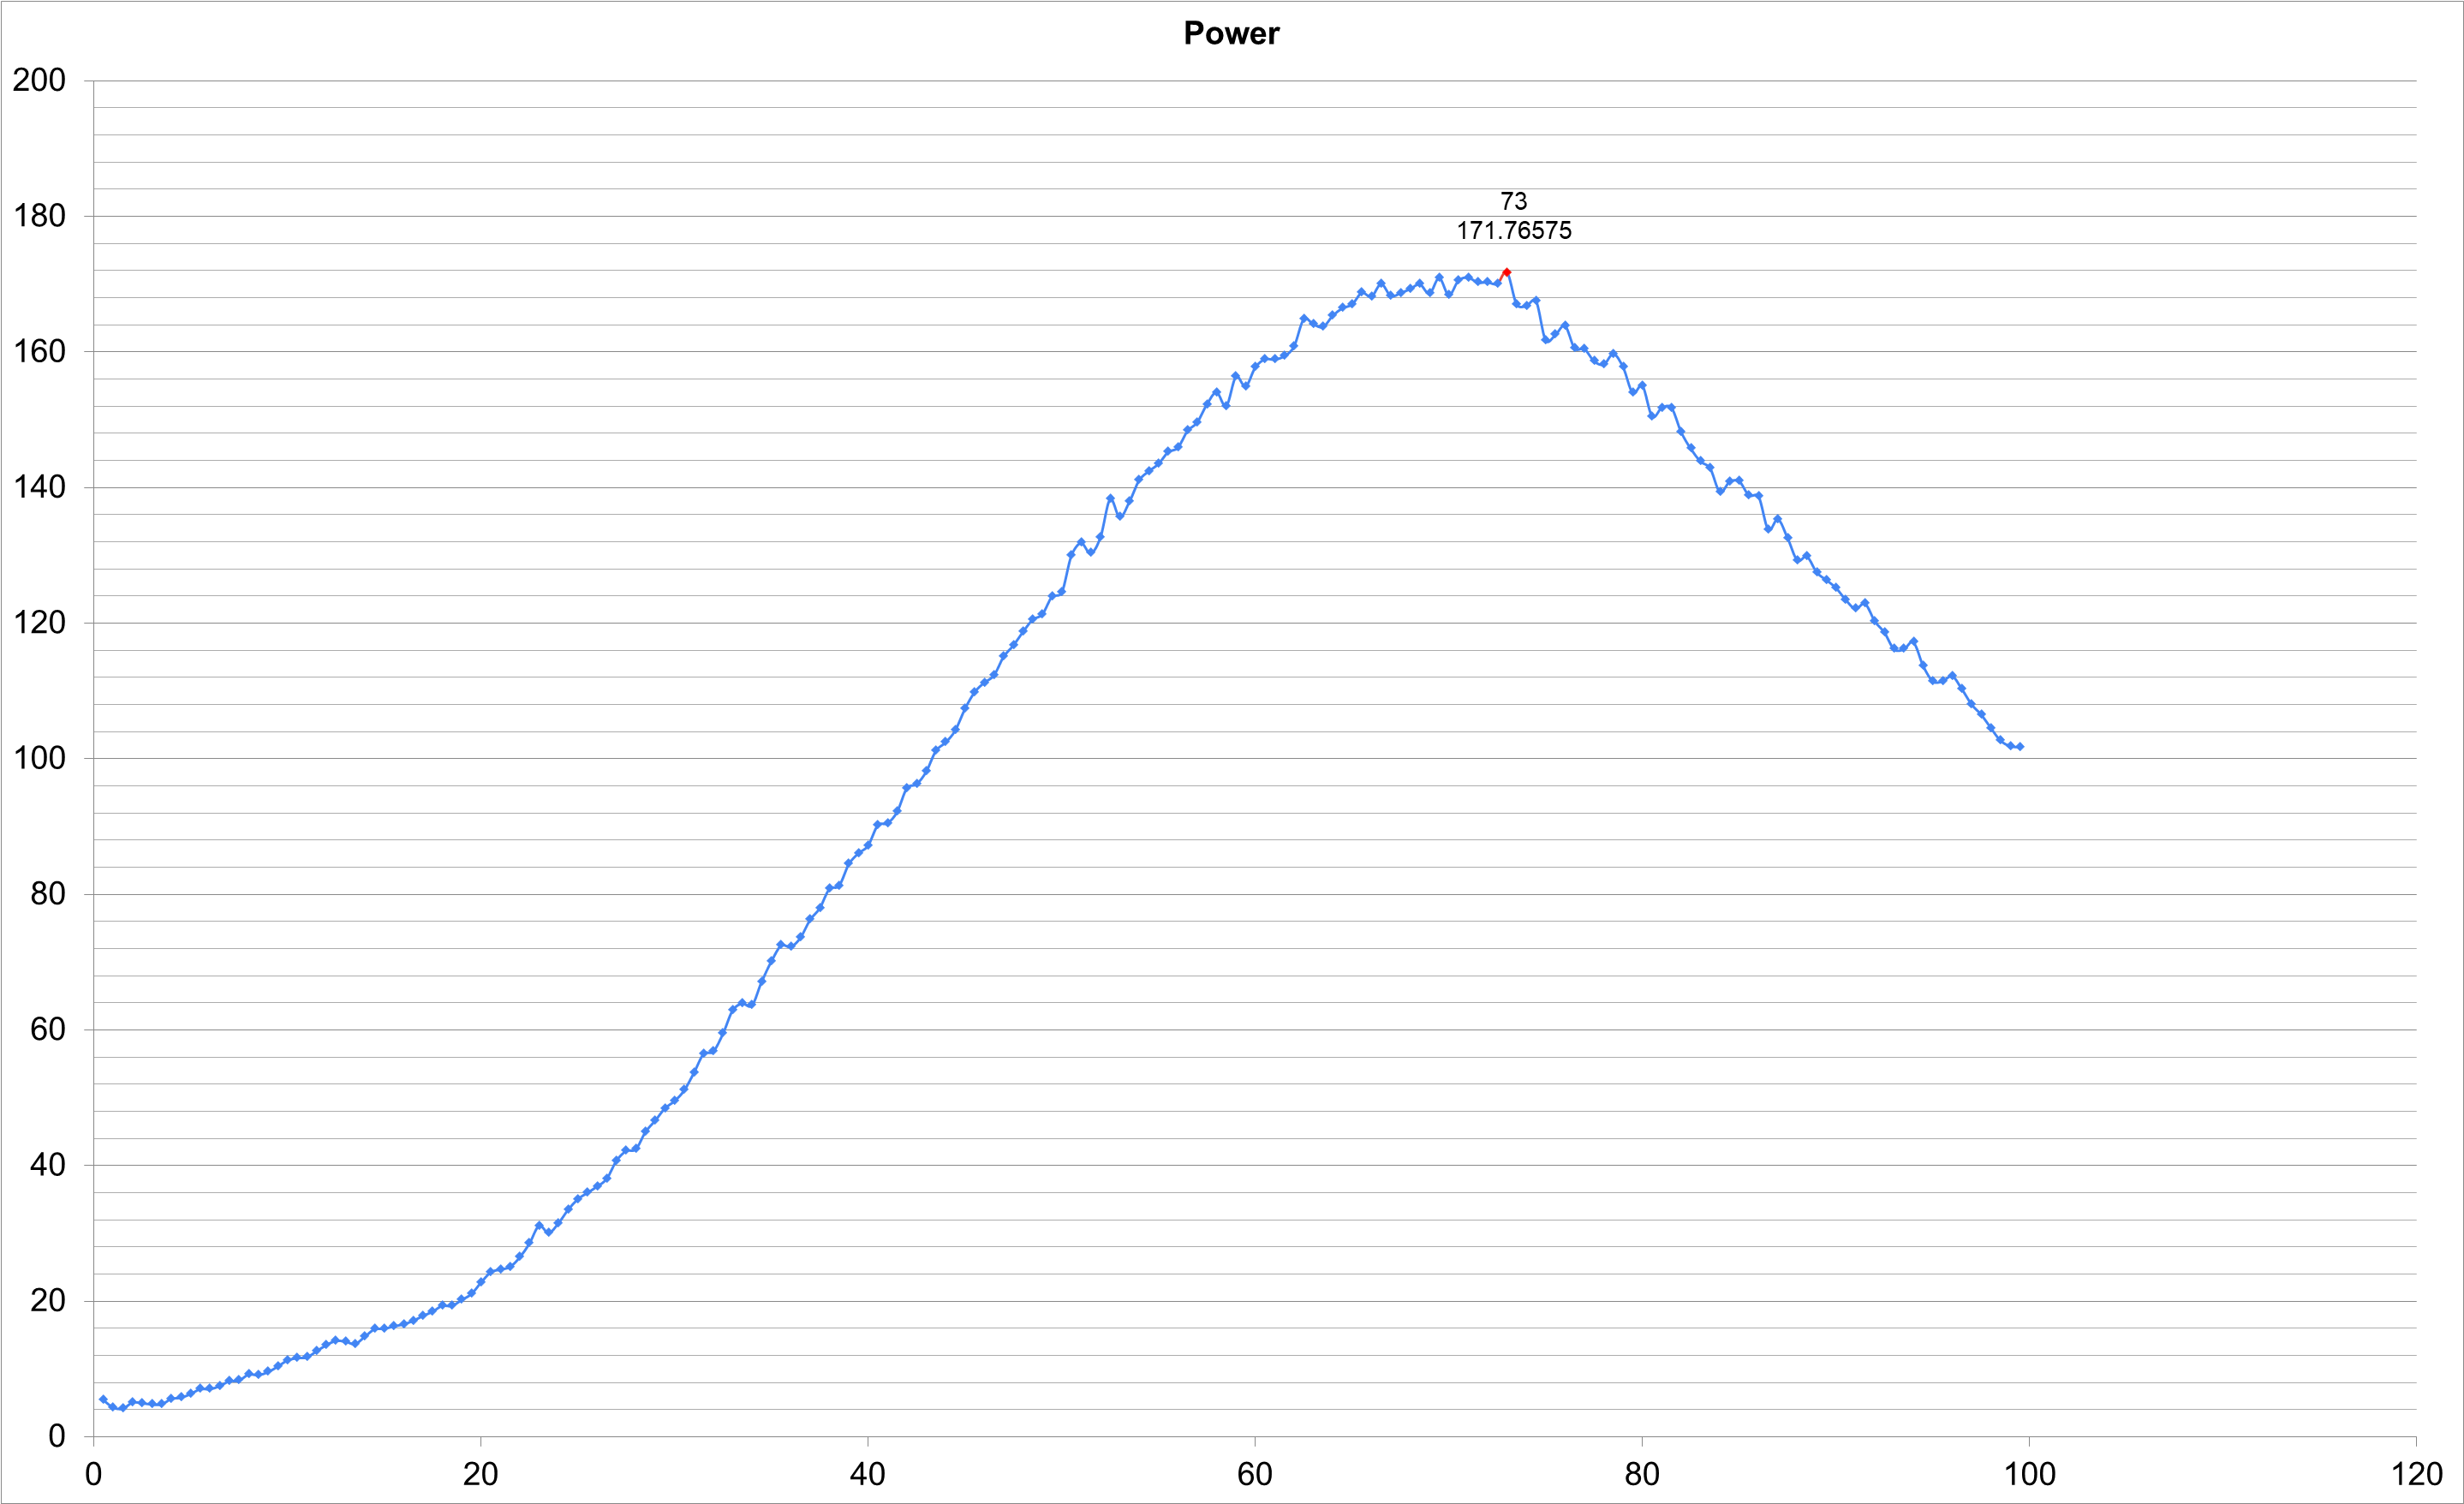
\includegraphics[width=1\linewidth]{imagenes/curva_panel_solar_por_esp32.png}
    \caption{Curva característica de panel solar a través de ESP32}
    \label{fig:curva_panel_esp32}
\end{figure}
(Texto debajo de imagen para corroborar espacio. Posible problema a futuro en formato, el cual no se esta pensando por ahora hasta terminar los escritos)

\chapter{Conclusiones}
\label{conclusiones}
Por último las conclusiones.





\begin{thebibliography}{}
  \bibitem{fundamental} Robert W. Erickson, Dragan Maksimovic {\em Fundamentals of
  Power Electronics} Second Edition 2001.
  
  \bibitem{power}  Ned Mohan, Tore M. Undeland {\em POWER ELECTRONICS Converters, Applications, and Design} Third edition 2003.


  \bibitem{ir2110web} International Rectifier {\em Application Note} AN978a.




\end{thebibliography}

%\bibliography{bibliografia}
%\bibliographystyle{babunsrt}




\appendix
\chapter{Código en C}
\label{Código en C}

\vspace{0.7cm}
\lstinputlisting[style=codigo,language=bash,caption=Método múltiple búsqueda]{codigo_fuente/ejemplo1.sh}
\vspace{0.7cm}

\chapter{Código para Google sheets}
\label{Código para Google sheets}


\vspace{0.7cm}
\lstinputlisting[style=codigo,language=bash,caption=Codigo de Apps Script]{codigo_fuente/google_sheets.sh}
\vspace{0.7cm}

%\chapter{Datos de Excel}
\label{Datos de Excel}

\vspace{0.7cm}
\lstinputlisting[style=codigo,language=bash,caption=ejemplo1.sh]{codigo_fuente/goo.sh}
\vspace{0.7cm}
\chapter{Circuito en KiCad}
\label{Circuito en KiCad}
\subsubsection{Esquemático}
\begin{figure}[H]
\begin{center}
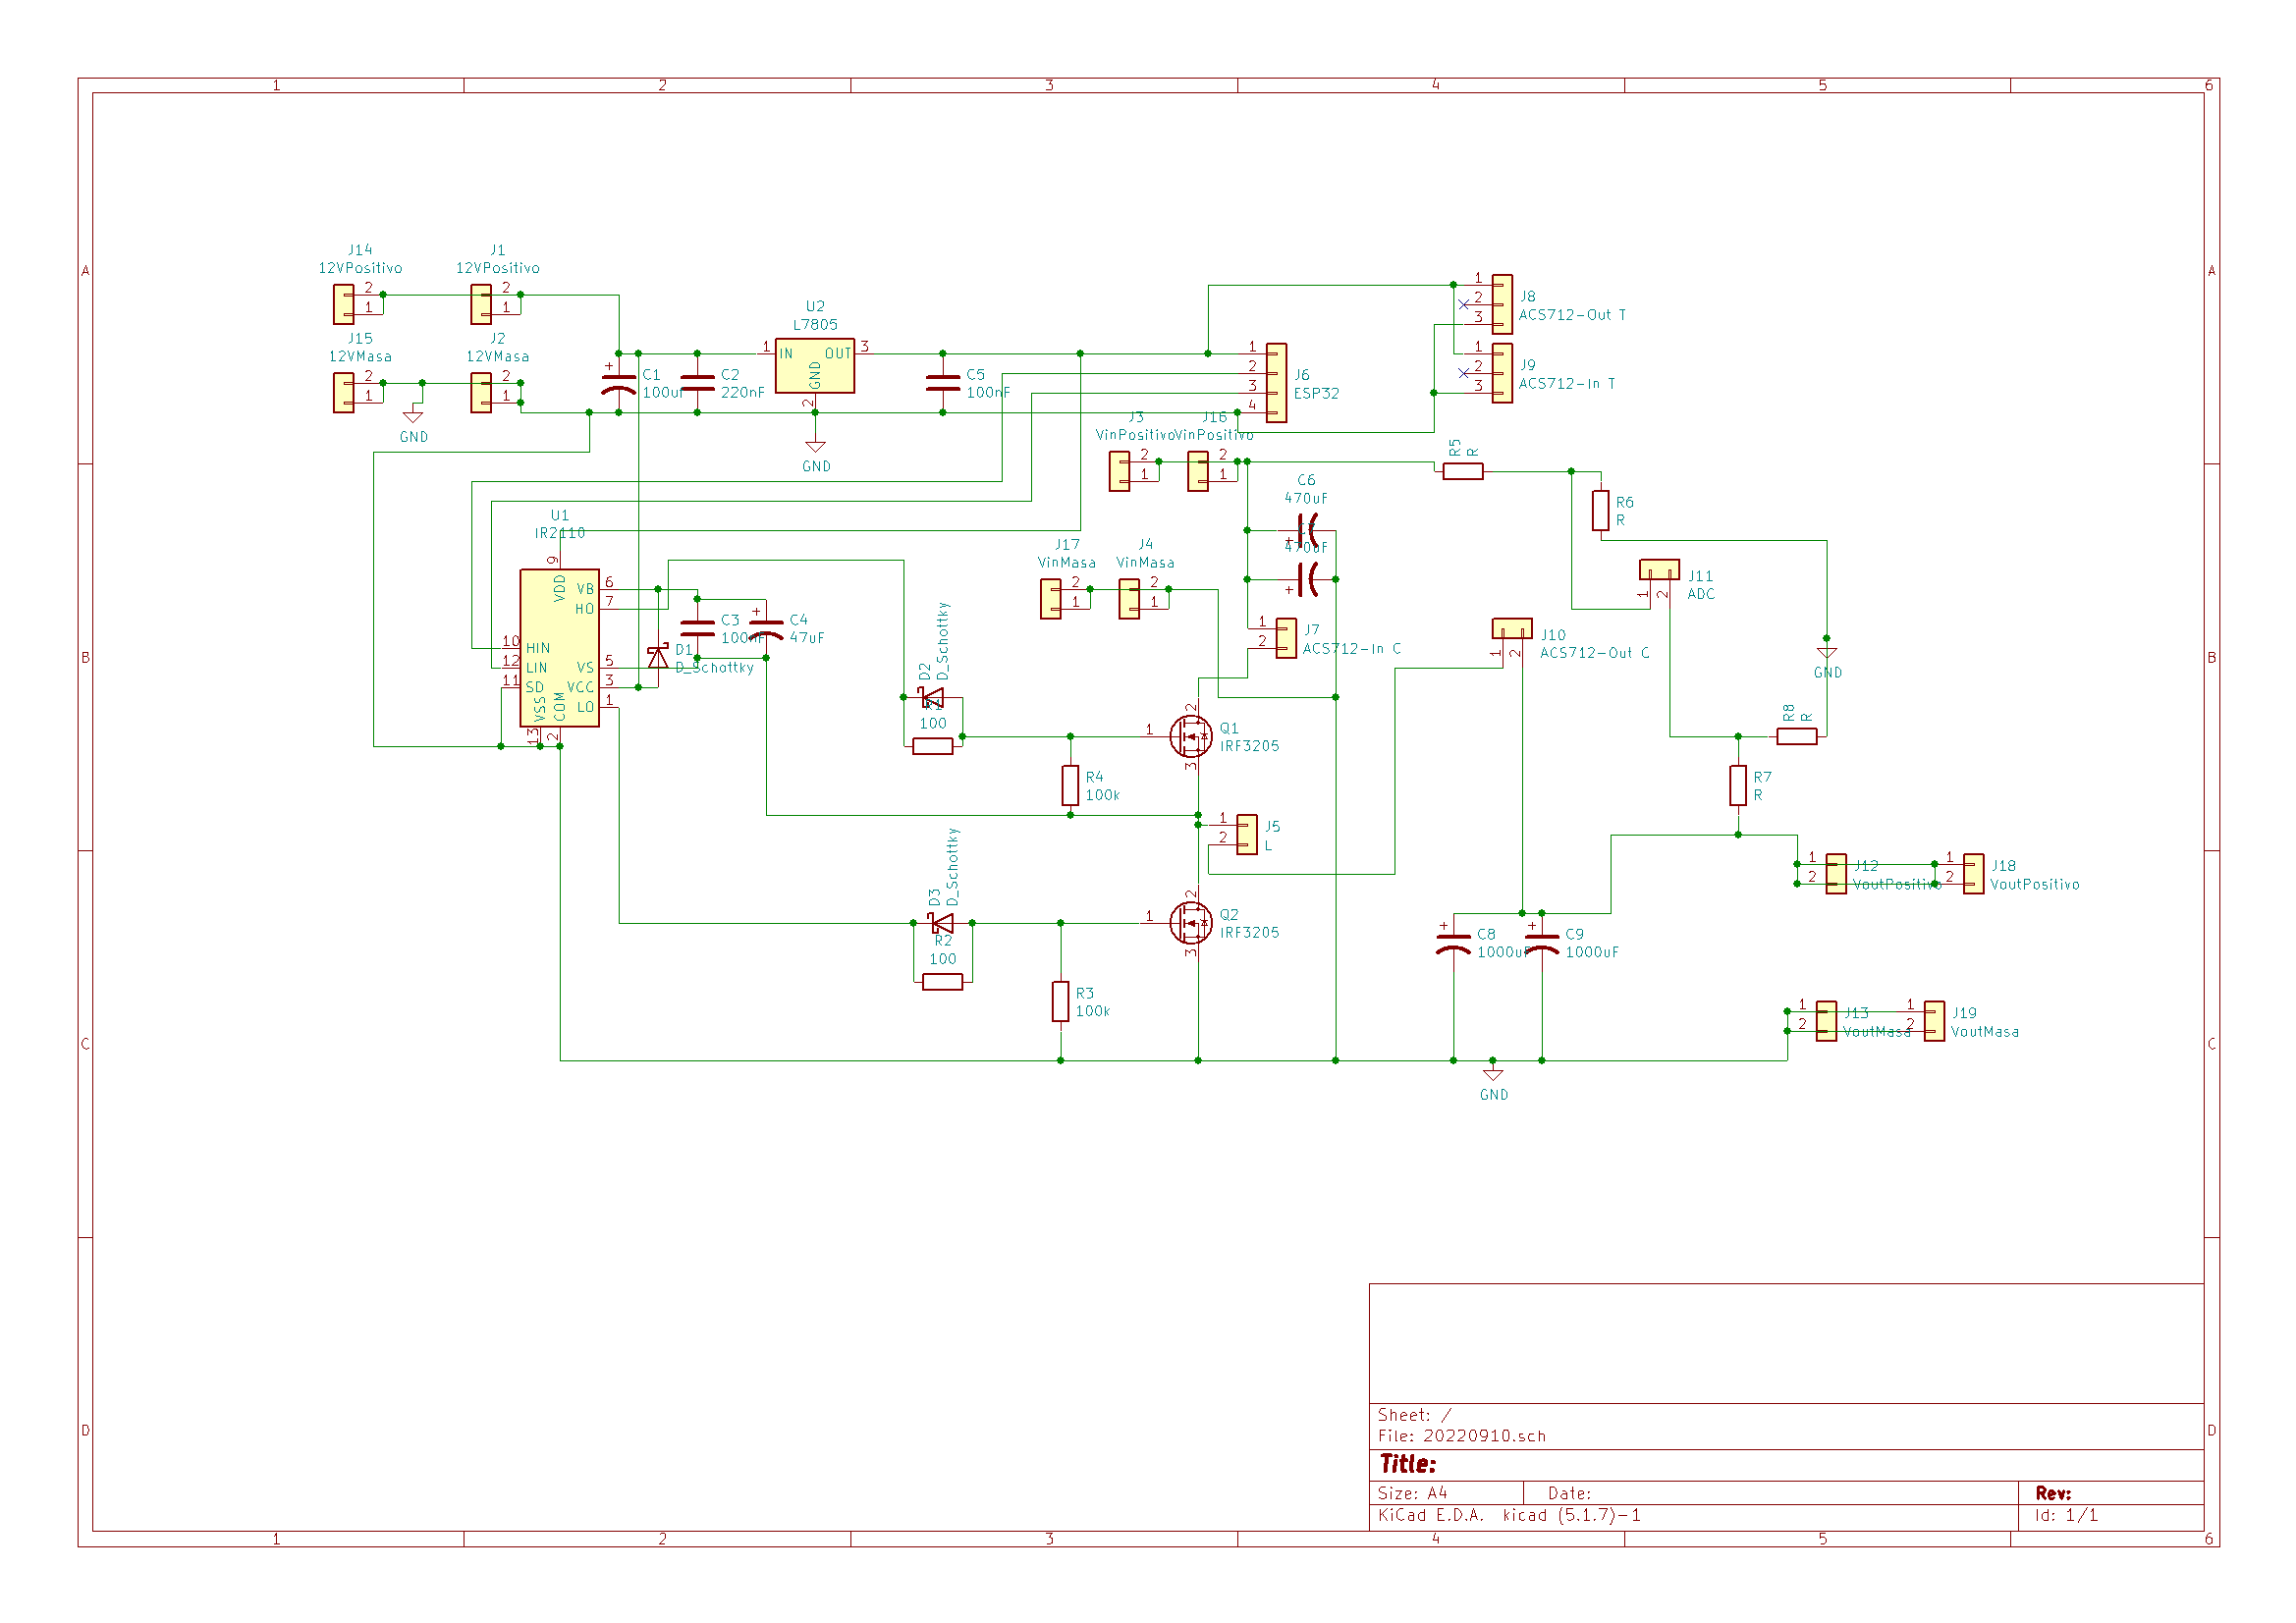
\includegraphics[width=1\linewidth,frame]{imagenes/kicadsquematics.png}
\caption{Esquematico en KiCad}
\label{fig:esquem_KiCad}
\end{center}
\end{figure}
\subsubsection{PCB}
\begin{figure}[H]
\begin{center}
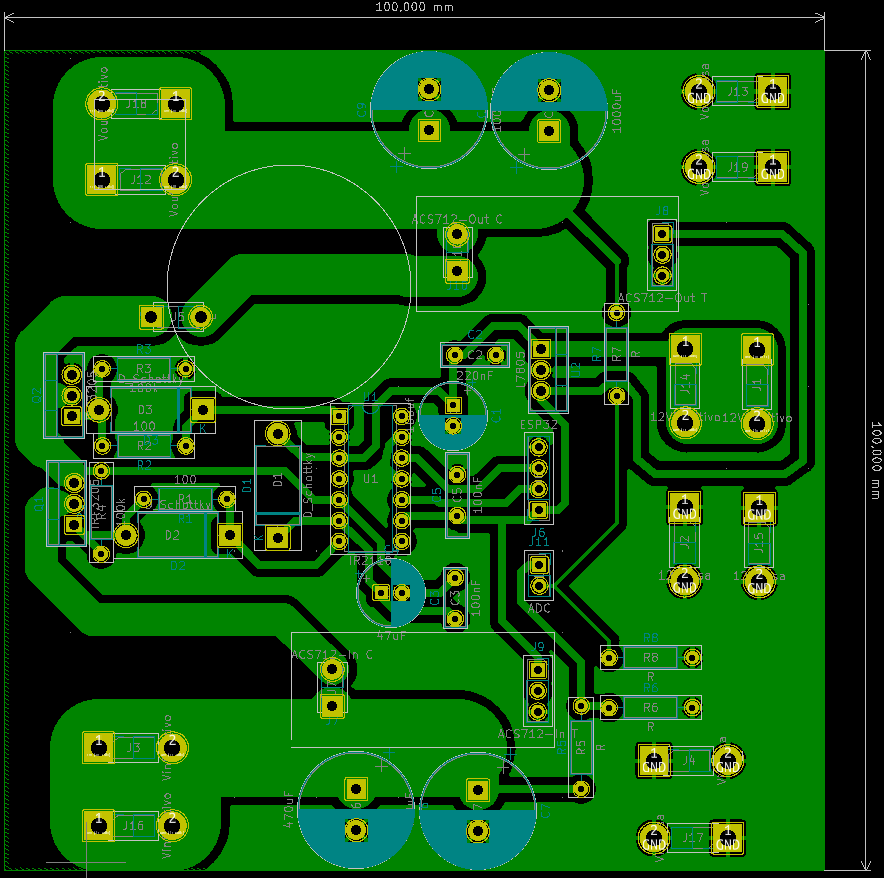
\includegraphics[width=1\linewidth,frame]{imagenes/pcbapendice.png}
\caption{Espero que se lea el PCB}
\label{fig:PCD_en_AP}
\end{center}
\end{figure}
\end{document}